\documentclass[11pt]{article}
\usepackage{amsmath, amssymb}
\usepackage{tikz}
\usepackage{pgfplots}
\usepackage{enumitem} % Added for custom enumerate labels
\pgfplotsset{compat=1.17}
\usetikzlibrary{matrix, trees, positioning, graphs, arrows.meta}

\begin{document}

\title{Assignment 7 --- Solutions for Parts 1, 3, and 4}
\author{Sean Balbale}
\date{\today}
\maketitle

\section*{Part 1: AVL Trees}

In this part we work with AVL Trees.

\subsection*{(a) AVL Tree Insertion}

We insert the keys in the order:
\[
    9,\,27,\,50,\,15,\,2,\,21,\,36.
\]
Below we detail the process step by step.

\textbf{Step 1.} \underline{Insert 9:}\\[2mm]
The tree is initially empty so 9 becomes the root.


\begin{center}
    \begin{tikzpicture}[level/.style={sibling distance=30mm, level distance=10mm}]
        \node {9};
    \end{tikzpicture}
\end{center}

\textbf{Step 2.} \underline{Insert 27:}\\[2mm]
Since $27>9$, insert 27 as the right child of 9.


\begin{center}
    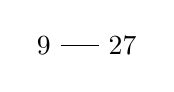
\begin{tikzpicture}[level/.style={sibling distance=30mm, level distance=10mm}]
        \node {9}
        child [grow=right] { node {27} };
    \end{tikzpicture}
\end{center}

\textbf{Step 3.} \underline{Insert 50:}\\[2mm]
Following BST rules, 50 is placed as the right child of 27. Now the tree appears as:
\[
    9 \rightarrow 27 \rightarrow 50.
\]
This yields an imbalance at 9 (balance factor $-2$) because the right subtree has height 2. This is a \textbf{Right-Right case} requiring a \textbf{left rotation} at node 9.


After rotation the tree becomes:
\[
    \begin{array}{c}
        \quad 27 \\[4mm]
        9 \quad\quad50
    \end{array}
\]


\begin{center}
    \begin{tikzpicture}[level/.style={sibling distance=30mm, level distance=10mm}]
        \node {27}
        child { node {9} }
        child { node {50} };
    \end{tikzpicture}
\end{center}

\textbf{Step 4.} \underline{Insert 15:}\\[2mm]
15 is less than 27 so we go left to 9; since $15>9$, insert 15 as the right child of 9.


\begin{center}
    \begin{tikzpicture}[level/.style={sibling distance=30mm, level distance=10mm}]
        \node {27}
        child { node {9}
                %   child { node {} [draw=none] }
                child { node {15} } }
        child { node {50} };
    \end{tikzpicture}
\end{center}

\textbf{Step 5.} \underline{Insert 2:}\\[2mm]
2 is less than 27; at 9, since $2<9$, insert 2 as the left child of 9.


\begin{center}
    \begin{tikzpicture}[level/.style={sibling distance=30mm, level distance=10mm}]
        \node {27}
        child { node {9}
                child { node {2} }
                child { node {15} } }
        child { node {50} };
    \end{tikzpicture}
\end{center}

\textbf{Step 6.} \underline{Insert 21:}\\[2mm]
Traverse: $21<27$ (go left), then at node 9: $21>9$ (go right) to node 15, and $21>15$ so insert as right child of 15.
Now the subtree rooted at 9 is:
\[
    \begin{array}{c}
        9               \\[2mm]
        2 \quad\quad 15 \\[2mm]
        \qquad\quad 21
    \end{array}
\]
This causes an imbalance at 27 (with a balance factor of $+2$) because node 9’s right subtree (via node 15) becomes taller than its left subtree. Moreover, node 9 has a balance factor of \(-1\) (right heavy). This is a \textbf{Left-Right (LR) case}. The remedy is to perform a \emph{double rotation}: first a left rotation at node 9, then a right rotation at node 27.


\underline{Left Rotation at 9:}\\[2mm]
The subtree rooted at 9 becomes:
\[
    \begin{array}{c}
        15              \\[2mm]
        9 \quad\quad 21 \\[2mm]
        2
    \end{array}
\]


\underline{Right Rotation at 27:}\\[2mm]
After this rotation the tree becomes:
\[
    \begin{array}{c}
        15              \\[4mm]
        9 \quad\quad 27 \\[4mm]
        2 \quad\quad 21 \quad\quad 50
    \end{array}
\]
Here 9 has left child 2, and 27 has left child 21 and right child 50.


\begin{center}
    \begin{tikzpicture}[level/.style={sibling distance=35mm, level distance=10mm}]
        \node {15}
        child { node {9}
                child { node {2} }
                %   child { node {} [draw=none] } 
            }
        child { node {27}
                child { node {21} }
                child { node {50} } };
    \end{tikzpicture}
\end{center}

\textbf{Step 7.} \underline{Insert 36:}\\[2mm]
Traverse: $36>15$, so move right to node 27; then $36>27$ so move to its right subtree; at 50, $36<50$, hence insert 36 as the left child of 50.


The final AVL tree is:
\[
    \begin{array}{c}
        \quad15                      \\[4mm]
        9 \quad\quad 27              \\[4mm]
        2\quad\quad 21 \quad\quad 50 \\[2mm]
        \qquad\quad\quad 36
    \end{array}
\]


\begin{center}
    \begin{tikzpicture}[level/.style={sibling distance=35mm, level distance=10mm}]
        \node {15}
        child { node {9}
                child { node {2} }
                child { node {} [draw=none] } }
        child { node {27}
                child { node {21} }
                child { node {50}
                        child { node {36} } } };
    \end{tikzpicture}
\end{center}

\vspace{4mm}
\textbf{Summary of Part (a):}\\[2mm]
After inserting 9, 27, 50, 15, 2, 21, and 36—with appropriate rotations (a left rotation at 9 and a double LR rotation at 27)—the final balanced AVL tree is as shown above.


\subsection*{(b) Deletion (Before Rebalancing)}
Consider the following given AVL tree:
\begin{center}
    \begin{tikzpicture}[
            level 1/.style={sibling distance=35mm, level distance=10mm},
            level 2/.style={sibling distance=30mm, level distance=10mm},
            level 3/.style={sibling distance=20mm, level distance=10mm}
        ]

        % Root node
        \node {5}
        child { % left subtree of 5
                node {3}
                child { % left subtree of 3
                        node {2}
                        child { node {1} }
                        child [missing] {} % no right child for 2
                    }
                child { % right subtree of 3
                        node {4}
                    }
            }
        child { % right subtree of 5
                node {10}
                child { % left subtree of 10
                        node {7}
                        child { node {6} }
                        child {
                                node {9}
                                child { node {8} }
                                child [missing] {} % no right child for 9
                            }
                    }
                child { % right subtree of 10
                        node {11}
                        child [missing] {} % no left child for 11
                        child { node {12} }
                    }
            };

    \end{tikzpicture}
\end{center}

After deleting node 5, we replace it with its inorder predecessor (node 4). The resulting tree is:

\begin{center}
    \begin{tikzpicture}[
            level 1/.style={sibling distance=50mm, level distance=10mm},
            level 2/.style={sibling distance=40mm, level distance=10mm},
            level 3/.style={sibling distance=25mm, level distance=10mm}
        ]

        % Root node
        \node {4}[sibling distance=50mm]  % Added explicit sibling distance
        child { % left subtree from node 4
                node {3}[sibling distance=35mm]  % Adjusted width
                child { % left subtree from node 3
                        node {2}
                        child { % left subtree from node 2
                                node {1}
                            }
                        child[missing] {}  % Fixed syntax
                    }
                child[missing] {}  % Fixed syntax
            }
        child { % right subtree from node 4
                node {10}[sibling distance=35mm]  % Adjusted width
                child { % left subtree from node 10
                        node {7}
                        child { % left child of node 7
                                node {6}
                            }
                        child { % right child of node 7
                                node {9}
                                child { % left child of node 9
                                        node {8}
                                    }
                                child[missing] {}  % Fixed syntax
                            }
                    }
                child { % right subtree from node 10
                        node {11}
                        child[missing] {}  % Fixed syntax
                        child {  % right child of node 11
                                node {12}
                            }
                    }
            };
    \end{tikzpicture}
\end{center}


\subsection*{(c) Rebalancing After Deletion}
In the above tree, notice that the left subtree of the root shows an imbalance: node \textbf{3} has a balance factor of +2. This indicates a left–left (LL) case, which can be corrected by performing a right rotation at node \textbf{3}. After the rotation, node \textbf{2} becomes the new parent for that subtree, with node \textbf{1} as its left child and node \textbf{3} as its right child. The right subtree remains unchanged.

Below is the rebalanced tree (balance factors are omitted):

\begin{center}
    \begin{tikzpicture}[
            level 1/.style={sibling distance=50mm, level distance=10mm},
            level 2/.style={sibling distance=40mm, level distance=10mm},
            level 3/.style={sibling distance=25mm, level distance=10mm}
        ]
        % Root node
        \node {4}
        child { % Left subtree after rebalancing
                node {2}
                child { % Left child of node 2
                        node {1}
                    }
                child { % Right child of node 2
                        node {3}
                    }
            }
        child { % Right subtree remains unchanged
                node {10}
                child { % Left subtree from node 10
                        node {7}
                        child { node {6} }
                        child { node {9}
                                child { node {8} }
                                child [missing] {}
                            }
                    }
                child { % Right subtree from node 10
                        node {11}
                        child [missing] {}
                        child { node {12} }
                    }
            };
    \end{tikzpicture}
\end{center}



\section*{Part 3: Graph Traversals}

\subsection*{Graph 1: Depth-First Search (DFS) Traversal}
Given a graph where the adjacency lists (neighbors) are arranged in ascending order, we perform a DFS starting at node 1. The DFS is implemented using a stack, and the procedure is as follows:

\subsection*{Procedure Overview}
\begin{enumerate}
    \item \textbf{Initialization:}
          \begin{itemize}
              \item Mark all nodes as unvisited.
              \item Create an empty stack.
              \item Push the start node (\textbf{1}) onto the stack and mark it as visited.
          \end{itemize}
    \item \textbf{While the stack is not empty:}
          \begin{itemize}
              \item Let the top of the stack be the current node.
              \item If the current node has an unvisited neighbor, push that neighbor onto the stack and mark it as visited.
              \item If the current node has no unvisited neighbors, pop it off the stack.
          \end{itemize}
\end{enumerate}

\subsection*{Step-by-Step DFS Execution}
\begin{enumerate}
    \item Start at node \textbf{1}.
          \textbf{Stack:} \([1]\)
          \textbf{Visited Order:} \(1\)
    \item From node 1, the neighbors (in ascending order) are: \(\{0,\,2,\,3,\,5\}\).
          The first unvisited neighbor is \textbf{0} → push 0.
          \textbf{Stack:} \([1,\,0]\)
          \textbf{Visited Order:} \(1,\,0\)
    \item At node 0, the only neighbor is \(\{1\}\), which is already visited → pop node 0.
          \textbf{Stack:} \([1]\)
    \item Back at node 1, the next unvisited neighbor is \textbf{2} → push 2.
          \textbf{Stack:} \([1,\,2]\)
          \textbf{Visited Order:} \(1,\,0,\,2\)
    \item At node 2, assume its neighbors are \(\{1,\,4,\,5\}\).
          The first unvisited neighbor is \textbf{4} → push 4.
          \textbf{Stack:} \([1,\,2,\,4]\)
          \textbf{Visited Order:} \(1,\,0,\,2,\,4\)
    \item At node 4, assume its neighbors are \(\{2,\,6\}\).
          The first unvisited neighbor is \textbf{6} → push 6.
          \textbf{Stack:} \([1,\,2,\,4,\,6]\)
          \textbf{Visited Order:} \(1,\,0,\,2,\,4,\,6\)
    \item At node 6, assume its neighbors are \(\{4,\,7\}\).
          The first unvisited neighbor is \textbf{7} → push 7.
          \textbf{Stack:} \([1,\,2,\,4,\,6,\,7]\)
          \textbf{Visited Order:} \(1,\,0,\,2,\,4,\,6,\,7\)
    \item At node 7, suppose its only neighbor is \(\{6\}\) (already visited) → pop node 7.
          \textbf{Stack:} \([1,\,2,\,4,\,6]\)
    \item Back at node 6, all neighbors have been visited → pop node 6.
          \textbf{Stack:} \([1,\,2,\,4]\)
    \item Back at node 4, all neighbors have been visited → pop node 4.
          \textbf{Stack:} \([1,\,2]\)
    \item Returning to node 2, the next unvisited neighbor is \textbf{5} → push 5.
          \textbf{Stack:} \([1,\,2,\,5]\)
          \textbf{Visited Order:} \(1,\,0,\,2,\,4,\,6,\,7,\,5\)
    \item At node 5, if its neighbors are \(\{1,\,2\}\) (both visited) → pop node 5.
          \textbf{Stack:} \([1,\,2]\)
    \item Back at node 2, no more unvisited neighbors → pop node 2.
          \textbf{Stack:} \([1]\)
    \item Back at node 1, the final unvisited neighbor is \textbf{3} → push 3.
          \textbf{Stack:} \([1,\,3]\)
          \textbf{Visited Order:} \(1,\,0,\,2,\,4,\,6,\,7,\,5,\,3\)
    \item At node 3, if the only neighbor is \(\{1\}\) (already visited) → pop node 3.
          \textbf{Stack:} \([1]\)
    \item Back at node 1, all neighbors are now visited → pop node 1.
          \textbf{Stack:} Empty.
\end{enumerate}

Thus, the DFS traversal order is:
\[
    \boxed{1 \to 0 \to 2 \to 4 \to 6 \to 7 \to 5 \to 3.}
\]

\subsection*{Visual Representation of DFS Order}
The following diagram illustrates the final order in which nodes are visited.

\begin{center}
    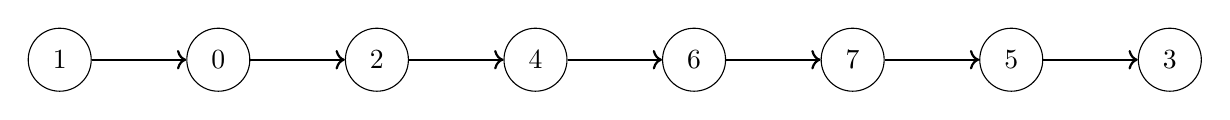
\begin{tikzpicture}[node distance=12mm, auto, every node/.style={draw, circle, minimum size=8mm}]
        \node (n1) {1};
        \node (n0) [right=of n1] {0};
        \node (n2) [right=of n0] {2};
        \node (n4) [right=of n2] {4};
        \node (n6) [right=of n4] {6};
        \node (n7) [right=of n6] {7};
        \node (n5) [right=of n7] {5};
        \node (n3) [right=of n5] {3};

        \draw[->, thick] (n1) -- (n0);
        \draw[->, thick] (n0) -- (n2);
        \draw[->, thick] (n2) -- (n4);
        \draw[->, thick] (n4) -- (n6);
        \draw[->, thick] (n6) -- (n7);
        \draw[->, thick] (n7) -- (n5);
        \draw[->, thick] (n5) -- (n3);
    \end{tikzpicture}
\end{center}



\textbf{Final DFS Visitation Order:} \(\boxed{1,\; 0,\; 2,\; 4,\; 6,\; 7,\; 5,\; 3.}\)


\subsection*{Graph 2: Breadth-First Search (BFS) Traversal}

In this example, we perform a BFS traversal on a graph starting from node 0. We assume that for each node the neighbors are considered in ascending numerical order. The BFS traversal is implemented using a queue as follows:



\textbf{BFS Procedure:}
\begin{enumerate}[label=\arabic*.]
    \item \textbf{Initialization:}
          \begin{itemize}
              \item Mark all nodes as unvisited.
              \item Create an empty queue.
              \item Enqueue the start node (node \textbf{0}) and mark it as visited.
          \end{itemize}
    \item \textbf{Iteration:} While the queue is not empty:
          \begin{itemize}
              \item Dequeue the front of the queue (let this be the current node).
              \item For each neighbor of the current node (in ascending order):
                    \begin{itemize}
                        \item If the neighbor is unvisited, mark it as visited and enqueue it.
                    \end{itemize}
          \end{itemize}
\end{enumerate}



\textbf{Step-by-Step Execution:}

\begin{enumerate}[label=\arabic*.]
    \item \textbf{Start at node 0:} Enqueue \(\mathbf{0}\). \\
          \(\textbf{Visited set: } \{0\}\) \\
          \(\textbf{Queue: } [0]\) \\
          \(\textbf{BFS Order: } 0\)
    \item \textbf{Dequeue 0:} Suppose the neighbors of 0 are \(\{1,2\}\). \\
          Enqueue \(1\) and \(2\) (both unvisited). \\
          \(\textbf{Visited set: } \{0,1,2\}\) \\
          \(\textbf{Queue: } [1,\,2]\) \\
          \(\textbf{BFS Order: } 0\)
    \item \textbf{Dequeue 1:} Suppose the neighbors of 1 are \(\{0,2,3,5\}\). \\
          Nodes \(0\) and \(2\) are already visited. \\
          Enqueue \(3\) and \(5\). \\
          \(\textbf{Visited set: } \{0,1,2,3,5\}\) \\
          \(\textbf{Queue: } [2,\,3,\,5]\) \\
          \(\textbf{BFS Order: } 0,\; 1\)
    \item \textbf{Dequeue 2:} Suppose the neighbors of 2 are \(\{1,4,6\}\). \\
          \(1\) is already visited; enqueue \(4\) and \(6\). \\
          \(\textbf{Visited set: } \{0,1,2,3,4,5,6\}\) \\
          \(\textbf{Queue: } [3,\,5,\,4,\,6]\) \\
          \(\textbf{BFS Order: } 0,\; 1,\; 2\)
    \item \textbf{Dequeue 3:} Suppose node 3's neighbor(s) are \(\{1\}\). \\
          \(1\) is already visited. \\
          \(\textbf{Queue: } [5,\,4,\,6]\) \\
          \(\textbf{BFS Order: } 0,\; 1,\; 2,\; 3\)
    \item \textbf{Dequeue 5:} Suppose the neighbors of 5 are \(\{1,2,3\}\). \\
          All are visited. \\
          \(\textbf{Queue: } [4,\,6]\) \\
          \(\textbf{BFS Order: } 0,\; 1,\; 2,\; 3,\; 5\)
    \item \textbf{Dequeue 4:} Suppose the neighbors of 4 are \(\{2\}\). \\
          \(2\) is visited. \\
          \(\textbf{Queue: } [6]\) \\
          \(\textbf{BFS Order: } 0,\; 1,\; 2,\; 3,\; 5,\; 4\)
    \item \textbf{Dequeue 6:} Suppose the neighbors of 6 are \(\{7\}\). \\
          Enqueue \(7\) (if unvisited). \\
          \(\textbf{Visited set: } \{0,1,2,3,4,5,6,7\}\) \\
          \(\textbf{Queue: } [7]\) \\
          \(\textbf{BFS Order: } 0,\; 1,\; 2,\; 3,\; 5,\; 4,\; 6\)
    \item \textbf{Dequeue 7:} Suppose node 7 has no unvisited neighbors. \\
          \(\textbf{Queue: } []\) \\
          \(\textbf{BFS Order: } 0,\; 1,\; 2,\; 3,\; 5,\; 4,\; 6,\; 7\)
\end{enumerate}



\textbf{Final BFS Visitation Order:}
\[
    \boxed{0 \to 1 \to 2 \to 3 \to 5 \to 4 \to 6 \to 7.}
\]



\textbf{Unreachable Vertices:} \\
Since every node \(\{0,1,2,3,4,5,6,7\}\) was visited during the BFS, there are no vertices unreachable from node 0.



\section*{Visual Representation of BFS Order}

The following TikZ diagram illustrates the BFS order using arrows:



\begin{center}
    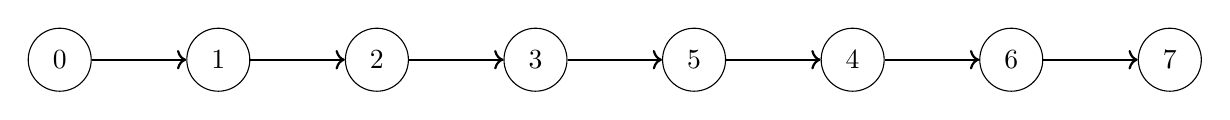
\begin{tikzpicture}[node distance=12mm, auto, every node/.style={draw, circle, minimum size=8mm}]
        \node (n0) {0};
        \node (n1) [right=of n0] {1};
        \node (n2) [right=of n1] {2};
        \node (n3) [right=of n2] {3};
        \node (n5) [right=of n3] {5};
        \node (n4) [right=of n5] {4};
        \node (n6) [right=of n4] {6};
        \node (n7) [right=of n6] {7};

        \draw[->, thick] (n0) -- (n1);
        \draw[->, thick] (n1) -- (n2);
        \draw[->, thick] (n2) -- (n3);
        \draw[->, thick] (n3) -- (n5);
        \draw[->, thick] (n5) -- (n4);
        \draw[->, thick] (n4) -- (n6);
        \draw[->, thick] (n6) -- (n7);
    \end{tikzpicture}
\end{center}



\textbf{Conclusion:} \\
The BFS traversal starting at node 0 visits the nodes in the order
\[
    \boxed{0,\; 1,\; 2,\; 3,\; 5,\; 4,\; 6,\; 7,}
\]
and all vertices of the graph are reachable from node 0.


\section{Part 4: Graph Representations}

Assume we are given a directed graph with 5 vertices, labeled \(0,1,2,3,4\), and the following edges (with weights):

\begin{itemize}
    \item \(0 \to 1\) (weight 3)
    \item \(0 \to 4\) (weight 4)
    \item \(4 \to 1\) (weight 1)
    \item \(1 \to 3\) (weight 3)
    \item \(2 \to 4\) (weight 1)
    \item \(2 \to 3\) (weight 7)
\end{itemize}



\subsection*{1. Graph Representations}

\subsubsection*{(a) Adjacency Matrix}

The adjacency matrix \(A = [a_{ij}]\) is constructed with rows and columns labeled \(0,1,2,3,4\) such that
\[
    a_{ij}=\begin{cases}
        \text{edge weight } w, & \text{if there is an edge } i \to j, \\
        0,                     & \text{otherwise.}
    \end{cases}
\]
For our graph, the matrix is:

\[
    \begin{array}{c|ccccc}
          & 0 & 1 & 2 & 3 & 4 \\ \hline
        0 & 0 & 3 & 0 & 0 & 4 \\
        1 & 0 & 0 & 0 & 3 & 0 \\
        2 & 0 & 0 & 0 & 7 & 1 \\
        3 & 0 & 0 & 0 & 0 & 0 \\
        4 & 0 & 1 & 0 & 0 & 0 \\
    \end{array}
\]




\subsubsection*{(b) Adjacency Graph (Adjacency List)}

The adjacency list stores for each vertex a linked list of all outgoing edges. For our graph the lists are:

\begin{itemize}
    \item \textbf{Vertex 0:} \(0 \to 1 \; (\text{weight }3),\; 0 \to 4 \; (\text{weight }4)\)
    \item \textbf{Vertex 1:} \(1 \to 3 \; (\text{weight }3)\)
    \item \textbf{Vertex 2:} \(2 \to 4 \; (\text{weight }1),\; 2 \to 3 \; (\text{weight }7)\)
    \item \textbf{Vertex 3:} No outgoing edges.
    \item \textbf{Vertex 4:} \(4 \to 1 \; (\text{weight }1)\)
\end{itemize}

Each edge node stores:
\begin{itemize}
    \item Destination vertex index: 2 bytes
    \item Edge weight: 2 bytes
    \item Pointer to the next edge: 4 bytes
\end{itemize}
Thus, each edge node uses \(2+2+4=8\) bytes.

Also, a vertex record (in the vertex array) stores:
\begin{itemize}
    \item Vertex index: 2 bytes
    \item Pointer to its edge list: 4 bytes
\end{itemize}
That is \(2+4=6\) bytes per vertex.



\subsection*{2. Memory Requirements}

We are given the following size assumptions:
\begin{itemize}
    \item Vertex index: 2 bytes
    \item Pointer: 4 bytes
    \item Edge weight: 2 bytes
\end{itemize}

\subsubsection*{(a) Directed Graph}

\paragraph{Adjacency Matrix:}
The matrix has \(n=5\) vertices, so there are \(5 \times 5 = 25\) entries.
\[
    \text{Total Memory} = 25 \times 2 = 50 \text{ bytes.}
\]

\paragraph{Adjacency List:}
\begin{itemize}
    \item \textbf{Vertex Array:} \(5 \text{ vertices} \times 6 \text{ bytes} = 30 \text{ bytes}.\)
    \item \textbf{Edge Nodes:} There are 6 edges. Each edge node uses 8 bytes.
          \[
              6 \times 8 = 48 \text{ bytes.}
          \]
\end{itemize}
So, the total memory for the adjacency list is:
\[
    30 + 48 = 78 \text{ bytes.}
\]

\subsubsection*{(b) Undirected Graph}

For an undirected graph, each edge is stored twice in the adjacency list.

\paragraph{Adjacency Matrix:}
The matrix remains unchanged:
\[
    25 \times 2 = 50 \text{ bytes.}
\]

\paragraph{Adjacency List:}
\begin{itemize}
    \item \textbf{Vertex Array:} Remains \(30\) bytes.
    \item \textbf{Edge Nodes:} Each of the original 6 edges appears twice, so there are \(6 \times 2 = 12\) edge nodes.
          \[
              12 \times 8 = 96 \text{ bytes.}
          \]
\end{itemize}
Thus, total memory is:
\[
    30 + 96 = 126 \text{ bytes.}
\]



\section*{Summary of Results}

\textbf{Directed Graph:}
\begin{itemize}
    \item \textbf{Adjacency Matrix:} \(50\) bytes.
    \item \textbf{Adjacency List:} \(78\) bytes.
\end{itemize}

\textbf{Undirected Graph:}
\begin{itemize}
    \item \textbf{Adjacency Matrix:} \(50\) bytes.
    \item \textbf{Adjacency List:} \(126\) bytes.
\end{itemize}

\end{document}
